\documentclass{beamer}
\usetheme{Madrid}
\usepackage{policyengine}
\usepackage{graphicx}
\usepackage{booktabs}

\title{Enhancing the CPS with Administrative Tax Data}
\subtitle{Machine Learning Meets Microsimulation}
\author[Woodruff \& Ghenis]{Nikhil Woodruff \& Max Ghenis}
\institute{PolicyEngine}
\date{National Tax Association Annual Conference\\November 14, 2024}

\begin{document}

\begin{frame}
    \titlepage
\end{frame}

\begin{frame}{The Challenge}
    \begin{itemize}
        \item Current Population Survey (CPS)
        \begin{itemize}
            \item Rich demographics, state ID, household structure
            \item But underreports income, especially at top
            \item Limited tax information
        \end{itemize}
        \pause
        \item IRS Public Use File (PUF)
        \begin{itemize}
            \item Accurate tax records from administrative data
            \item But no demographics beyond age/sex
            \item No state ID
            \item Protected by strict confidentiality rules
        \end{itemize}
    \end{itemize}
\end{frame}

\begin{frame}{Key Innovation: Open Dataset with PUF Quality}
    \begin{itemize}
        \item First openly available dataset integrating CPS and PUF
        \item No confidentiality restrictions
        \item Enables:
        \begin{itemize}
            \item Transparent policy analysis
            \item Integration with other tools
            \item Community contributions and validation
        \end{itemize}
        \item Powers PolicyEngine's microsimulation platform
    \end{itemize}
\end{frame}

\begin{frame}{Our Approach}
    \begin{itemize}
        \item Generate synthetic tax variables from PUF using:
        \begin{itemize}
            \item Quantile regression forests to learn distributions
            \item Match to CPS demographic variables
        \end{itemize}
        \pause
        \item Stack synthetic records with original CPS
        \pause
        \item Calculate taxes and benefits via microsimulation
        \pause
        \item Optimize weights against 570 targets:
        \begin{itemize}
            \item IRS Statistics of Income income bins
            \item Program participation totals
            \item Single-year age population counts
        \end{itemize}
    \end{itemize}
\end{frame}

\begin{frame}{Validation: Administrative Targets}
    \begin{itemize}
        \item Enhanced CPS outperforms source datasets:
        \begin{itemize}
            \item 63\% of targets vs original CPS
            \item 71\% of targets vs PUF
        \end{itemize}
    \end{itemize}
\end{frame}

\begin{frame}{Validation: Inequality Measures}
    \begin{itemize}
        \item Tax unit income inequality matches IRS data
        \begin{table}
            \centering
            \begin{table}
                \centering
                \begin{table}[h]
    \centering
    \caption{Key tax unit-level distributional metrics}
    \label{tab:tax_unit_metrics}
    \begin{tabular}{lrrr}
    \toprule
    Metric & CPS & Enhanced CPS & PUF \\
    \midrule
    Gini coefficient & 0.495 & 0.572 & 0.570 \\
    Top 10\% share & 0.361 & 0.425 & 0.410 \\
    Top 1\% share & 0.085 & 0.154 & 0.150 \\
    \bottomrule
    \end{tabular}
\end{table}

            \end{table}
        \end{table}
    \end{itemize}
\end{frame}

\begin{frame}{Validation: Top Rate Reform}
    \begin{itemize}
        \item Biden's 2025 budget: raise top rate to 39.6\% above \$400k
    \end{itemize}
    \begin{table}
        \centering
        \begin{table}[h]
    \centering
    \caption{Revenue projections from top rate increase (37\% to 39.6\%)}
    \label{tab:top_rate_reform}
    \begin{tabular}{llll}
    \toprule
    Dataset & Revenue Impact (\$B) & Affected Tax Units (M) & Avg Tax Increase (\$) \\
    \midrule
    CPS & [TBC] & [TBC] & [TBC] \\
    Enhanced CPS & [TBC] & [TBC] & [TBC] \\
    PUF & [TBC] & [TBC] & [TBC] \\
    \bottomrule
    \end{tabular}
\end{table}

    \end{table}
\end{frame}

\begin{frame}{Advanced ML Methods}
    \begin{itemize}
        \item Quantile regression forests (QRF) for:
        \begin{itemize}
            \item Tax variable imputation from PUF
            \item Housing costs from ACS
            \item Prior year earnings from ASEC panel
        \end{itemize}
        \pause
        \item Dropout-regularized gradient descent for:
        \begin{itemize}
            \item Weight optimization
            \item Preventing overfitting
            \item Handling sparse subgroups
        \end{itemize}
    \end{itemize}
\end{frame}

\begin{frame}{The PolicyEngine Platform}
    \begin{figure}
        \centering
        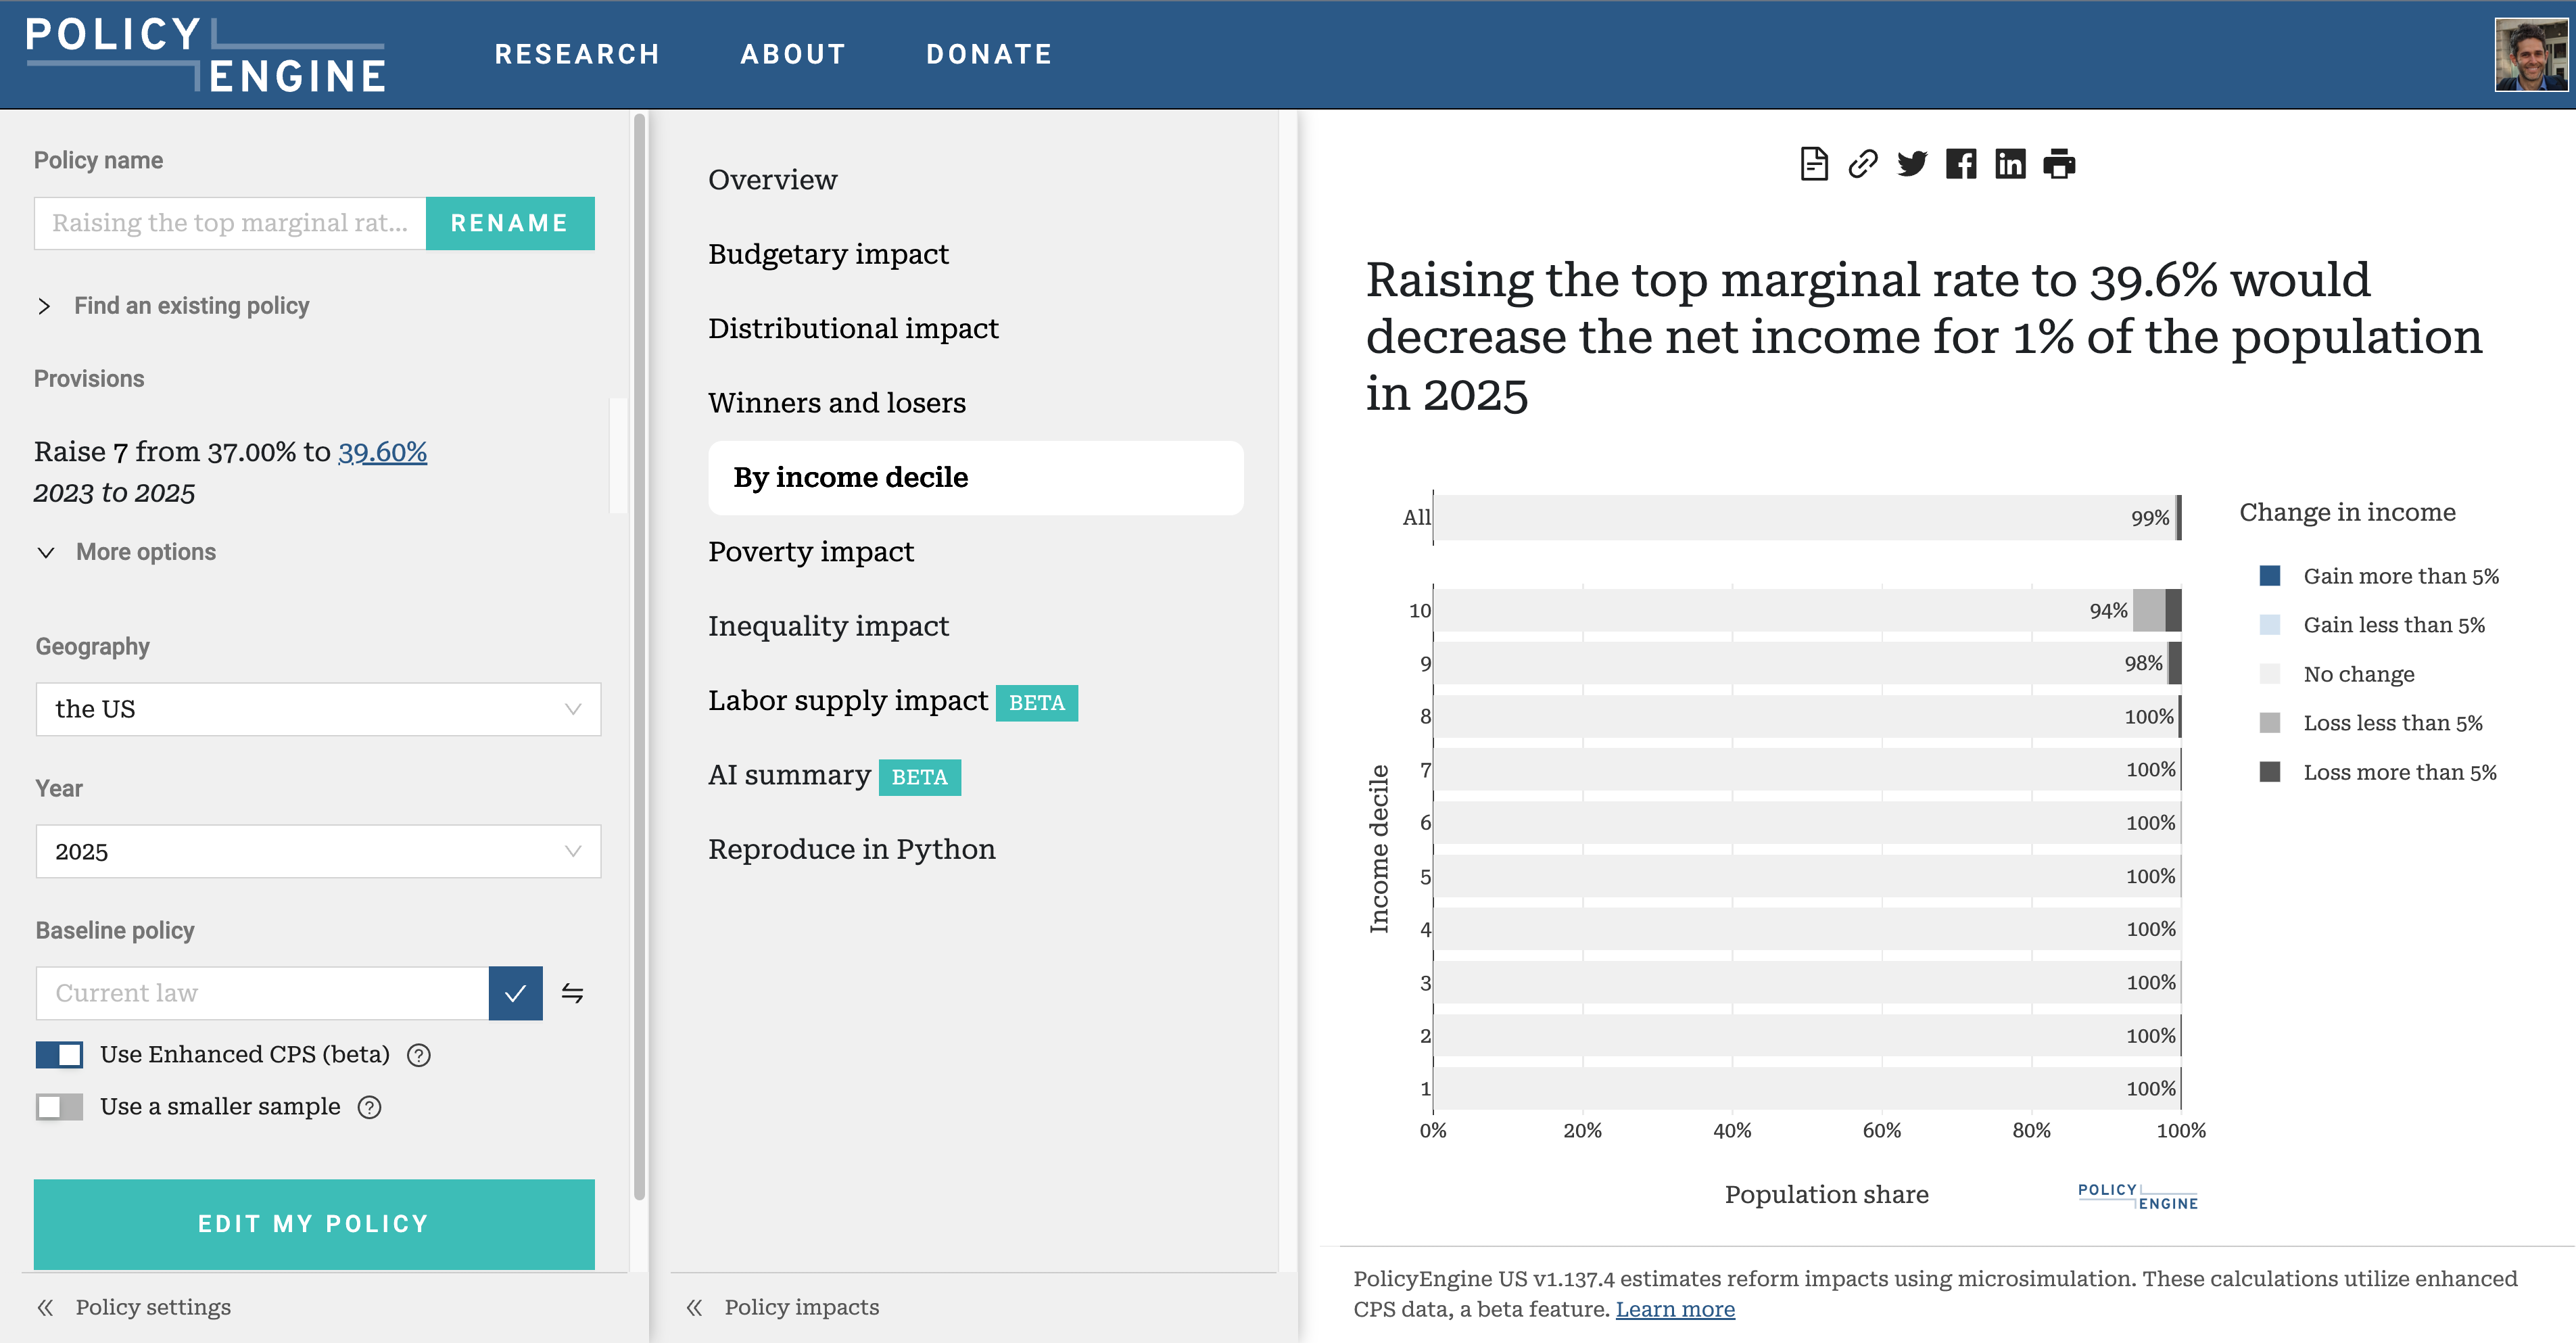
\includegraphics[width=0.8\textwidth]{../../paper/figures/policyengine_results.png}
        \caption{Screenshot of PolicyEngine's US tax and benefit calculator}
    \end{figure}
    \begin{itemize}
        \item Web interface for policy analysis
        \item Powered by enhanced CPS
        \item Instant distributional impacts
    \end{itemize}
\end{frame}

\begin{frame}{Open Access}
    \begin{itemize}
        \item All code open source
        \begin{itemize}
            \item github.com/PolicyEngine/policyengine-us-data
            \item Reproducible enhancement pipeline
            \item Automatic validation dashboard
        \end{itemize}
        \pause
        \item Use through Python package or web interface
        \pause
        \item Growing community of users:
        \begin{itemize}
            \item Academic researchers
            \item Think tanks
            \item Government agencies
        \end{itemize}
    \end{itemize}
\end{frame}

\begin{frame}{Next Steps}
    \begin{itemize}
        \item Geographic extensions:
        \begin{itemize}
            \item Congressional district weights
            \item State-specific calibration
            \item County-level synthetic data
        \end{itemize}
        \pause
        \item Methodological improvements:
        \begin{itemize}
            \item Time series validation
            \item Uncertainty quantification
            \item Alternative ML architectures
        \end{itemize}
    \end{itemize}
\end{frame}

\begin{frame}{Thank You}
    \begin{itemize}
        \item Paper: github.com/PolicyEngine/policyengine-us-data/paper
        \item Code: github.com/PolicyEngine/policyengine-us-data
        \item Web app: policyengine.org
        \item Contact: max@policyengine.org
    \end{itemize}
\end{frame}

\end{document}